% !TeX TS-program = latexmk % | dvisvgm --pdf --exact --font-format=woff --zoom=-1 %.pdf | txs:///view-log | txs:///view-pdf 
\documentclass{standalone}
\usepackage{tikzducks}

\pagecolor{gray!20!white}

\begin{document}
	
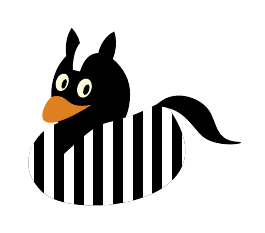
\begin{tikzpicture}
	\path (0.1,0.1) rectangle (2.75,2.35);
	\begin{pgfinterruptboundingbox}
	\begin{scope}[yshift=-6]
		\clip[rotate=-5] (0.68,2.38) ellipse (0.3 and 0.4);
		\fill[black,rotate=-5] (0.28,2.26) ellipse (0.3 and 0.4);
	\end{scope}
	\duck[
		body=black,
		stripes={\stripes[color=white,distance=0.25,width=0.125,rotate=0,initialx=0.06]},
		horsetail=black,
		mohican=white
	]
	\begin{scope}[yshift=-5,xshift=1]
		\clip[rotate=-5] (0.68,2.38) ellipse (0.3 and 0.4);
		\fill[black,rotate=-5] (1.06,2.2) ellipse (0.3 and 0.4);
	\end{scope}
	\end{pgfinterruptboundingbox}
\end{tikzpicture}
	
\end{document}